%!TEX root = ../Project.tex

\subsection{Allocation algorithm}

% Writeup from the meeting with JC

% [@todo nice and modular]

\subsubsection{Human aspects}
\label{sec:algo_humanaspects}

During the research period, discussions with academic and administrative staff
in both pilot departments revealed that the current method of module
allocation is not particularly complex. With several hundred students being
allocated modules by a few different members of staff, it is impossible to
produce a uniformly ``fair'' allocation of modules to students. The staff
simply try their best to allocate as many high choices as possible.

For example, the History department allocates between one and four modules to
each of their students. The administrators and academic staff recounted how,
during the allocation period, every surface in the departmental office would
be covered with sheets of paper (one or two per student, numbering over one
thousand in total) on which students had ranked their modules. The department
would attempt to perform the best allocation, though clearly they had no way
of verifying mathematically that the allocation was optimal.

With this information in hand, I began to investigate how the departments and
students saw each of the choices, as this influences what the aim of the
solver will be. A pattern began to emerge of which choices were good and which
were bad:

\begin{itemize}
  \item A first choice is perfect -- if every student received every one of
        their first choices, they could not complain about the allocation.
  \item A second or third choice is alright -- a student would not be too
        displeased to be taking their second or third choice module.
  \item A fourth or fifth choice should be avoided where possible, but is not
        a show-stopper.
  \item One would expect a student who was being made to take their sixth or
        lower choice to be fairly unhappy.
\end{itemize}

While there are an astounding number of different allocations
possible\footnote{In the History department's pilot run there were
approximately 18000 binary variables, or $2^{18000}$ different allocations},
it is trivial to sum a score for each allocation as follows:

$$
c_1(x_1) + c_2(x_2) + c_3(x_3) ...
$$

...where $x_i$ is the number of $i^{th}$ choices that that allocation created.
The coefficient $c_i$ multiplied by the number of $i^{th}$ choices indicates a
penalty applied by the system -- this penalty increases depending on how
negative that choice is deemed to be. While not particularly complex,
instructing the solver to minimise this score would maximise the number of
highly ranked choices.

The Archaeology department commented that they could not recall ever having to
give a student their fourth choice or below, as they are a fairly small
department (with less than 3\% of all York undergraduates). This means that
they can normally find sufficient capacity to offer every student their first,
second or third choice.

The History department is far larger than Archaeology, and additionally
reserves a number of spaces on their modules for visiting students. This will
place a strain on the allocation, as the department anticipates there will
most likely not be enough space on the most popular modules for every student
that wants to take them. They aim to give their students ``two from five'' --
that is to say, for a student ranking a group of eight modules, the two that
they are allocated were among their top five choices.

Eliciting these ideas explicitly from the departments was one of the harder
parts of interacting with the project clients, and in fact the final
coefficients used were not confirmed until a project group meeting on 23
February, just two weeks before the allocation was due to be performed.

\subsubsection{Variables}

As mentioned previously, the binary variables in this system are one for every
\studmod pair indicating that an allocation is possible. The variable is a 0
if no allocation is made, or a 1 otherwise. These variables are written as
$x_{S,M}$ when discussing the objective function and constraints.
Additionally, there is one binary variable for every module indicating whether
that module is to be taught that academic year. This allows the system to
indicate whether a better allocation can be produced by disregarding an
unpopular module. These variables are written $y_{M}$ in this document.

\subsubsection{Objective function}

The basic idea behind the objective function was discovered through
discussions with departments. For each allocation, every \studmod pair is
included in the objective function. In this example, \texttt{rank()} returns
the coefficient related to the rank that that student gave to that module:

$$
\displaystyle\sum \{x_{S,M} \times rank(S,M)\}
$$

During testing, I made use of the solver's ability to write out a \texttt{.lp}
file. This section makes use of extracts from the file to demonstrate the
objective function and constraints. The file begins:

\begin{lstlisting}
Maximize
  + 15 ax563fake_34 + 2 ax563fake_39 + 30 ax563fake_30 + 235 ax563fake_43
   + 60 ax563fake_44 + 120 ax563fake_38 + 6 ax563fake_35
   + 1000 ax563fake_36 + 2048 ax563fake_41 + 480 ax563fake_33
...
\end{lstlisting}

Deconstructing the first term in this linear function, \texttt{15} is the
coefficient related to the rank that student \texttt{ax563fake} gave to the
module with database ID \texttt{34}. \texttt{ax563fake\_34} is the solver's
representation of a binary variable which is set to 1 if the student takes the
module. I made the decision to apply larger coefficients to better rankings
and to maximise the function as I felt this was more intuitive from a
maintainability perspective. The final coefficients used in the objective
function were decided with the help of the departments and are shown in
Figure~\ref{gurobi_coeff}.

\subsubsection{Constraints}

Originally, the hard constraints on the optimisation problem were as follows:

\begin{itemize}
  \item The lower cap on a module (a module will not run with fewer than the
        required number of students)
  \item The upper cap on a module (a staff member is not able to provide the
        required quality of teaching to more than the maximum number of students)
  \item The number of credits a student must take from a particular group of
        modules (each student must have exactly the same workload as their
        peers)
\end{itemize}

Two additional constraints were added at the request of the History
department. The first is that they have one case where students can not take
both module A and module B. The second is a constraint which attempts to
ensure that each student is given an approximately equally good allocation.
These constraints are explained here.

\noindent{\textbf{Correct number of students in a module}}

Each module has a minimum and a maximum number of students that must be placed
in it to ensure that modules are approximately the same size. The first part
of this constraint is simple; a student cannot take a module if it does
contain the minimum number of students. For every \studmod binary variable a
hard constraint is applied indicating that a student can take a module
($x_{S,M}=1$) if and only if the module is running ($y_M=1$):

$$
\forall x_{S,M} \quad x_{S,M} \leq y_M
$$

The second part of this constraint is slightly more complex; if a module is
running, it must have the minimum number of students. Alternatively this can
be thought of as ``if the module does not run (so $y_M=0$), we do not care
what the class size is'' and therefore the constraint vanishes. This is
expressed as:

$$
y_M \times module\_min(M) \leq \displaystyle\sum x_{S,M}
$$

The final part is again quite simple. The number of students allocated to a
module must always be less than the maximum size of the module, no matter
what:

$$
\displaystyle\sum x_{S,M} \leq module\_max(M)
$$

The idea that each module must have the correct number of students is
expressed as three different types of constraint in the \texttt{.lp} file.
Recall that \texttt{ax563fake\_34} is a binary variable indicating whether the
student is allocated the module, and note that \texttt{moduledma34} is a
binary variable indicating whether the module is run that year. The following
extract from that file demonstrates that:

\begin{enumerate}
  \item student \texttt{ax563fake} can only take module \texttt{34} if it is running
  \item module \texttt{34} must have a minimum of 14 students
  \item module \texttt{34} must have a maximum of 18 students
\end{enumerate}

\begin{lstlisting}
Subject To
 modrunning_ax563fake_34: ax563fake_34 - moduledma34 <= 0
 classmin_34: ax563fake_34 + lz907fake_34 + kf123fake_34 + cz325fake_34
   + qr385fake_34 + sv078fake_34 + zn998fake_34 + eb795fake_34
   ...
   - 14 moduledma34 >= 0
 classmax_34: ax563fake_34 + lz907fake_34 + kf123fake_34 + cz325fake_34
   + qr385fake_34 + sv078fake_34 + zn998fake_34 + eb795fake_34
   ...
   <= 18
\end{lstlisting}

\noindent{\textbf{Correct number of credits per group, per student}}

Each student must be allocated the correct number of credits from every group
that they rank modules from. As mentioned when describing the database schema
(Section~\ref{developmentdatabasestructure}), each module is worth a certain
number of credits. Each group contains one or more modules, and has a number
of credits that must be allocated. Additionally, students have the ability to
declare that they are taking an elective module in a different department, and
so should not be allocated the full quota of credits. For every student we
apply the following constraint to every group:

$$
group\_credits(G) - elective\_credits(G,S) = \displaystyle\sum_{M \in G} x_{S,M} \times module\_credits(M)
$$

In the \texttt{.lp} file, this constraint is expressed for student
\texttt{ax563fake} and the group with ID \texttt{20} as:

\begin{lstlisting}
credits_ax563fake_20: 40 ax563fake_40 + 40 ax563fake_34 + 40 ax563fake_39
  + 40 ax563fake_30 + 40 ax563fake_43 + 40 ax563fake_37 + 40 ax563fake_45
  ...
  + 40 ax563fake_41 + 40 ax563fake_33 = 40
\end{lstlisting}

This extract represents a student with no elective modules being required to
take 40 credits from a group consisting of several modules. The solver will
allocate exactly one module from this group, as they are all worth 40 credits.

\noindent{\textbf{Specific departmental constraints}}

The History department stated that two of their modules were exclusive (i.e.
no student could take both). In the solver, this constraint (applied to all
students) is specified as:

$$
x_{S,M_1} + x_{S,M_2} \leq 1
$$

This is because if both modules are allocated, the left hand side will be 2.
Though in the case when a student is allocated either module (or neither of
them), the constraint is satisfied.

\noindent{\textbf{Equity across students}}

This additional hard constraint was added later in the implementation process,
as departments enquired whether it would be possible to ensure that every
student received approximately the same ``goodness of allocation''. The
constraint is described as equity across students because it attempts to
ensure that the system does not give any single student an allocation that
would make them much better off than any other student.

The constraint is created under the assumption that there will always be at
least one student who receives the first choices they request. A hard
constraint is added to each student so that the sum of the ranks that they
gave to the modules they were eventually allocated is less than some ``equity
cap'' that is defined by the department when the allocation is performed.

$$
\displaystyle\sum (x_{S,M} \times rank(S,M)) \leq equity\_cap
$$

Ideally this cap would be normalised because students take different numbers
of modules and so can have vastly different sums of ranks, but unfortunately
there was not sufficient time to implement this constraint to that level of
detail. As a workaround, the department set different ``equity caps'' on
different types of student to ensure equity.

\subsubsection{Gurobi Optimizer}

From the research in Section~\ref{sec:researchilp}, Gurobi appears the more
suitable choice of solver for this application. The allocation problem can be
implemented directly in the application using the Java interface, so it will
hopefully be more quickly understood by a University Java developer.
Additionally, it was found by Mittelmann to be faster than SCIP, though this
may not be relevant with the relatively small model sizes this application
will produce.

% Generated using R:
% points <- c(2048, 1000, 480, 235, 120, 60, 30, 15, 6, 2, 1, 1, 0, 0, 0)
% plot(points, xlab="Rank of module", ylab="Coefficient", main="Graph of coefficient against module ranks")
% lines(points)
% dev.copy(pdf, '/path/to/gurobi_coefficients.pdf')
% dev.off()

\begin{figure}
  \begin{center}
    \fbox{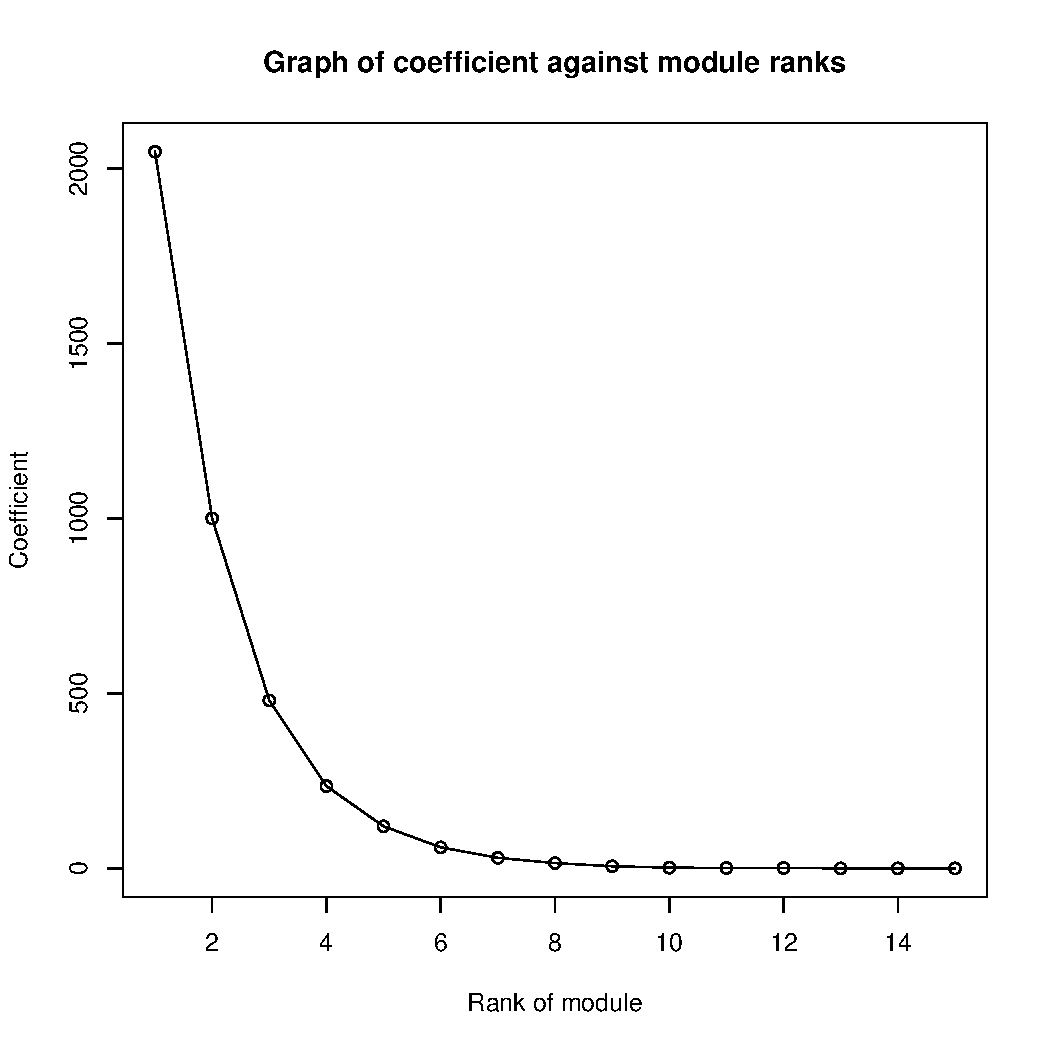
\includegraphics[width=0.6\linewidth]{images/gurobi_coefficients.pdf}}
  \end{center}
  \caption{Coefficients used in the solver's objective function}
  \label{gurobi_coeff}
\end{figure}

Figure~\ref{gurobi_coeff} shows a graph of the coefficients that were used in
the objective function. It demonstrates that the information provided to the
solver approximates the imaginary score function a staff member might use when
allocating modules manually.

To begin with, Gurobi's Python interface was used
to prototype the model. As the project implementer is more familiar with
Python than with Java, it was faster to prototype using the Python interface.
Additionally, there is less development overhead required with Python (i.e. no
compilation necessary). Once the Gurobi solver was working correctly on static
data using the Python interface, it was transferred to the application,
changed to using the Java interface and integrated with the application
database. A copy of the Gurobi code is included in
Appendix~\ref{sec:gurobicode}.
